% Load the institute for communications engineering document class
\documentclass[chair=lut]{ICEthesis} % options for the chair are lnt (default), lut or cod

%!TEX root = ../main.tex
\usepackage[
    shortcuts,       % enable short forms like gls etc.
    acronym,         % enable auto-generation of the acronym glossary
    nomain,          % disable the main glossary
    section=chapter, % set the glossary title format to be like a chapter (alternatives are section, subsection, etc.)
    toc=true,        % show in table of contents
]{glossaries}
\glsenableentrycount % enable counting of the references, otherwise \cgls does the same as \gls

\usepackage{siunitx} % for \Si, \SI and \SIRange
\sisetup{
    range-units=single, % only print unit once, e.g. 2 to 4 ◦C
    range-phrase=--, % print a range with dashes instead of "to"
    scientific-notation = engineering, % format numbers as 1.2x10^3 (with exponents multiple of 3)
}
\DeclareSIUnit\baud{Bd} % define Baud

\usepackage[capitalize]{cleveref} % \cref

%!TEX root = ../main.tex
\graphicspath{ {figs/} } % set the figures folder such that we don't need to write it in all includegraphics commands

% Macros:
\newcommand{\eq}[1]{Equation (\ref{#1})} % \eg{eq:golomb}  --> Equation (2.15)
\newcommand{\eref}[1]{(\ref{#1})}        % \eg{eq:golomb}  --> (2.15)
\newcommand{\fig}[1]{Figure \ref{#1}}    % \fig{fig:golomb}--> Figure 2.15
\newcommand{\tab}[1]{Table \ref{#1}}     % \tab{tab:lala}  --> Table 2.15
\newtheorem{prop}{Proposition}

% Abbreviations
\newcommand{\equivalent}{\triangleq}
\newcommand{\given}{\:\!\vert\:\!}

%!TEX root = ../main.tex
\makeglossaries % has to come first
%
% Example:
% \newacronym{xy}{XY}{Full Text}
% where xy is what you write in \[c]gls commands, XY is the acronym written in the text
% and "Full Text" is what is written out on the first occasion.
% The "c" prefix means "counting". It takes a bit of processing time, but it will figure out if an acronym is
% only used once and in that case only print the long version and not introduce the acronym at all.
%
% To use these acronyms in the text:
% \cgls{xy} % regular call, writes it out the first time, acronym otherwise
% \cglspl{xy} % same as \cgls, but plural form
% \Gls{xy} % same as \cgls, but capitalized
% \Glspl{xy} % same as \cglspl, but capitalized
% \acrshort{xy} same as \gls, but always prints the short version, even if it's the first time in the document
% \acrlong{xy} same as \gls, but always prints the long version
% \acrfull{xy} same as \gls, but always prints the long and short version
%
% Usually you don't include the glossary in a paper, but for a thesis you should.
% To do that:
% * put \makeglossaries in the preamble
% * call this after the first latex run: "cd build && makeglossaries main" and run latex again
% * add \printglossary where it should be
%
\newacronym{awgn}{AWGN}{additive white gaussian noise}
%
\newacronym{ber}{BER}{bit error rate}
%
\newacronym{snr} {SNR} {signal-to-noise ratio}
%
\newacronym{ask} {ASK} {amplitude shift keying}
%
\newacronym{qam} {QAM} {quadrature amplitude modulation}
%
\newacronym{dl} {DL} {deep learning}
%
\newacronym{nn} {NN} {neural network}
%
\newacronym{sgd} {SGD} {stochastic gradient descent}
%
\newacronym{mi} {MI} {mutual information}
%
\newacronym{mb} {MB} {Maxwell-Boltzmann}
\usepackage{physics}
\newtheorem{theorem}{Theorem}

\begin{document}
% ##########
% Title page
% ##########
\ICEtitle{Master's Thesis} % Thesis type (Master's Thesis or Bachelor's Thesis)
    {Thesis Title}
    {Student Name}
    {Dipl.-Ing.~Advisor}
    {München, Month Year}
    { % your data
        Student Name\\
        Streetname Number\\
        ZIP München\\
        your.email@addre.ss
    }

\ICErecht{Student Name}{München, xx.xx.20xx}

\cleardoubleemptypage % start new double page / neue Doppelseite



% ########################################
% Table of Contents / Inhaltsverzeichnis
% ########################################
% roman page numbering, starting with page number 1
\setcounter{page}{1}
\pagenumbering{roman}

\tableofcontents
% list of figures and list of tables is optional, feel free to comment if you like
%\listoffigures
%\listoftables
\cleardoubleemptypage


% ########
% Chapters
% ########
% arabic page numbering, starting with page number 1
\setcounter{page}{1}
\pagenumbering{arabic}

% Include chapters
%!TEX root = ../main.tex
\addchap{Abstract}\label{chap:abstract} % basically chapter*, but keeps the chapter in the table of contents
The abstract comes here.

%!TEX root = ../main.tex
\chapter{Introduction}\label{chap:introduction}

The constant demand for higher capacity digital links has motivated the development of communication schemes which approach closer and closer the analytical limit of the channel capacity. According to the definition of channel capacity, sending a single bit per time-frequency slot is inefficient. For this reason, higher-order modulations like \cgls{ask} or \cgls{qam} are used for better efficiency. Under these modulation schemes, the receiver handles more than two signal points per real dimension --- the set of spacial signal points is known as constellation. However, these schemes present a constant-width gap to the capacity limit. This is due to the usage of both uniform and discrete probability distributions for the occurrence of the constellation points. While it is not possible to move away from the discrete distributions because of the digital nature of the communication, constellations with specific non-uniform distributions and optimized spatial locations can lead to further capacity improvements. 

Constellation shaping thus, is a technique which seeks to optimize the distribution of the transmit symbols. Furthermore, this optimization unfolds into the improvement of the constellation points' location, their occurrence probability or both simultaneously. The first is known as geometric shaping while the latter is known as probabilistic shaping. In both cases, the goal is to maximize the \cgls{mi} of the channel input X and output Y, which we denote with $I(X;Y)$, by optimizing the constellation. This optimization problem arises from the definition of channel capacity $C$:
\begin{align}
\label{eqn:capacity}
	C = \max_{p(X)} I(X;Y).
\end{align}

Currently, the optimal $p(x)$ has only been found for specific channels, such as the \cgls{awgn}, since knowledge of the channel distribution $p(y|x)$ is required. Still, solving (\ref{eqn:capacity}) can become mathematically intractable despite knowing $p(y|x)$.

Here is where the use of machine-learning is key for finding constellations which maximize $I(X;Y)$, without analytical knowledge of the channel or with very complex $p(y|x)$. As shown in \cite{O'Shea}, the complete communication system can be interpreted as an autoencoder. This approach tackles the physical layer by optimizing the end-to-end performance instead of the performance of the individual components. To achieve this, the loss function, against which the trainable parameters will be optimized, must be carefully selected. What is more, geometric shaping under the autoencoder framework has been already performed in \cite{O'Shea} and \cite{Jones}. Still, learning the optimal probability distribution presents an additional challenge --- the statistics of the training set are altered during the learning of the probability distribution making numerical approximations unprecise. \cite{Stark} and \cite{Aref} address this problem with different proposals. Their results show that the joint application of probabilistic and geometric shaping outperform the PS-QAM scheme from \cite{Boecherer} and approach the limit to within 0.1 dB in the AWGN channel. Nonetheless, the existence of multiple and apparently different architectures invites for a comparative study. Consequently, in this work we implement and discuss the architectures proposed by \cite{Stark} and \cite{Aref}.

The rest of this document is organized as follows. Chapter 2, Preliminaries, presents the fundamentals of classical Probabilistic constellation systems as well as of autoencoder systems. Chapter 3, Contribution, presents a comparative study of two autoencoder architectures which can perform joint porbabilistic and geometric constellation shaping and highlights their limitations. Chapter, Conclusions, 4 wraps-up this work.

%!TEX root = ../main.tex
\chapter{Preliminaries}\label{chap:preliminaries}
\section{Probabilistic Constellation Shaping}
In this section our goal is to present the capacity limitations of the commonly used \cgls{ask} and \cgls{qam} modulation schemes. These schemes are penalized for two reasons:
\begin{enumerate}
\item They use uniform probability densities.
\item The constellation points are equidistant.
\end{enumerate}
In the following we explain the nature of these penalties.
\subsection{Introduction}
We begin with an important result from Information theory. Under a second-moment constraint, also known as power constraint, the probability distribution which maximizes the differential entropy is the Gaussian distribution, denoted with $p_G$. We thus have
\begin{align}
\label{eqn:max_entropy_scalar}
	h(X) \leq \dfrac{1}{2} \log \left(2 \pi e \sigma^2 \right)
\end{align}
where $\sigma^2 = \mathbb{E}[X^2]$, and with equality if and only if $X$ is Gaussian-distributed. More generally in the multi-dimensional case we have  
\begin{align}
\label{eqn:max_entropy_n}
	h(\underline{X}) \leq \dfrac{1}{2} \log \left((2 \pi e)^n |\textbf{Q}_{\underline{X}}| \right)
\end{align}
where we have considered a random column vector $\underline{X}$ of dimension n, mean $\mathbb{E}[\underline{X}]= \underline{m}$ and covariance matrix
\begin{align}
	\textbf{Q}_{\underline{X}}  = \mathbb{E}[(\underline{X} - \underline{m})(\underline{X} - \underline{m})^\intercal]
\end{align}
and equality in (\ref{eqn:max_entropy_n}) if only if the elements of $\underline{X}$ are jointly Gaussian.\\

\begin{figure}[ht]
\centering
\begin{tikzpicture}
    \node(src){};
    \node[circle, draw, inner sep=0cm]at (4,0) (plus){$+$};
	
	\node at (4,1.5)(z){$Z\sim\mathcal{N}(0,N)$};

	\draw[-latex] (src) --  (plus) node[midway,above] {$X\sim\mathcal{N}(0, P)$};
	\draw[-latex] (plus) -- node[midway,above] {$Y$} (6,0);	
	
	\draw[-latex](z)--(plus);
\end{tikzpicture}
\end{figure}

Lets now consider an \cgls{awgn} channel with Gaussian input $X$, of zero mean and variance $P$; Gaussian noise $Z$, of zero mean and variance $N$; and output $Y$; i.e. $Y = X + Z$. %A visual representation of the \cgls{awgn} channel is provided in Figure \ref{}.

Furthermore, the capacity of the \cgls{awgn} is
\begin{align}
\label{eqn:awgn_cap}
	C(P) &= \max\limits_{P_X:\mathbb{E}[X^2] \leq P} \mathbb{I}(X;Y)\\
	& = \max\limits_{P_X:\mathbb{E}[X^2] \leq P}[h(Y) - h(Y \vert X)]\\
	& = \dfrac{1}{2} \log (2 \pi e (P+N)) - \dfrac{1}{2} \log (2 \pi e N)\\
	& = \dfrac{1}{2} \log \left(1 + \dfrac{P}{N} \right). 
\end{align}
We can express the mutual information
\begin{align}
\label{eqn:MI}
	\mathbb{I}(X;Y) = h(Y) - h(Y \vert X)
\end{align}
in two parts, the differential entropy of the output and the conditional differential entropy of the output given the input.
We expand the second term as
\begin{align}
	h(Y \vert X) &= h(Y - X \vert X) \\
	& = h(Z \vert X)\\
	& = h(Z) = \dfrac{1}{2} \log \left(2 \pi e \sigma^2 \right)
\end{align}
and observe that the term $h(Y \vert X)$ does not depend on how $X$ is distributed. In contrast, $h(Y)$ does depend on how $X$ is distributed by
\begin{align}
	p_Y(y) = \int_{-\infty}^{\infty} p_X(X)p_Z(y -x) \,dx = (p_X \star p_Z)(y).
\end{align}
To circumvent the fact that it is difficult to find a closed-form expression of $h(Y)$, we make use of the information divergence as
\begin{align}
\label{eqn:hy_ce}
	h(Y) \overset{\text{(a)}}{=}  h(Y_G) - \mathbb{D}(p_Y \Vert p_G)
\end{align}
where (a) arises from the fact that $\mathbb{X}(p_X \Vert p_G) = h(Y_G)$ if and only if $p_X$ has zero mean and variance P as $p_G$. (\ref{eqn:hy_ce}) is very useful as it allows us to express the differential entropy of the output in terms of the information divergence between $p_G$ and any other distribution by means of the cross entropy. 

Now we can rewrite \ref{eqn:MI} as
\begin{align}
	\mathbb{I}(X;Y) &= h(Y) - h(Y \vert X)\\
	& = h(Y) - h(Z)\\
	& = h(Y_G) - \mathbb{D}(p_Y \Vert p_G) - h(Z)\\
	& = [h(Y_G) - h(Z)] - \mathbb{D}(p_Y \Vert p_G)\\
	& = C(P/\sigma^2) - \mathbb{D}(p_Y \Vert p_G).
\label{eq:C_minus_D}
\end{align}
This last result indicates that the loss of MI when using a distribution $P_X$ different than $P_G$ is the informational divergence $\mathbb{D}(p_Y \Vert p_G)$. In other words, if the Gaussian distribution is not used, the capacity penalty is characterized by $\mathbb{D}(p_Y \Vert p_G)$.\\

\subsection{Capacity Gap for Uniform Continuous Input}
\begin{figure}[ht!]
\centering
\begin{tikzpicture}
    \node(src){};
    \node[circle, draw, inner sep=0cm]at (4,0) (plus){$+$};
	
	\node at (4,1.5)(z){$Z\sim\mathcal{N}(0,N)$};

	\draw[-latex] (src) --  (plus) node[midway,above] {$X\sim\mathcal{U}\left[-A, A\right]$};
	\draw[-latex] (plus) -- node[midway,above] {$Y$} (6,0);	
	
	\draw[-latex](z)--(plus);
\end{tikzpicture}
\end{figure}
We would like now to understand how far a uniform distribution is from (\ref{eqn:max_entropy_scalar}). To do this, we will follow the approach presented in \cite{BoechererCM} to lower bound the MI. Start by defining $X_u$ as a uniformly distributed input on the interval $[-A, A]$ where A is carefully chosen so that $\mathbb{E}[{X_u}^2] = P$. The corresponding output is $Y_u$ and we proceed
\begin{align}
	\mathbb{I}(X_u;Y_u) &= C(\text{snr}) - \mathbb{D}(p_{Y_u} \Vert p_{Y_G})\\
	& \geq C(\text{snr}) - \mathbb{D}(p_{X_u} \Vert p_{X_G})\\
	& = C(\text{snr}) -[h(X_G) - h(X_u)]\\
	& = C(\text{snr}) - \dfrac{1}{2} \log_{2} \left(\dfrac{\pi e}{6}\right).
	\label{eqn:gap}
\end{align}
In Figure \ref{fig:capacity_gap} we display the derived lower bound and observe that the capacity loss, originated from the use of a uniform input density, is never more than $\dfrac{1}{2}\log_2\dfrac{\pi e}{6}$ independent of the \cgls{snr}.
\begin{figure}
	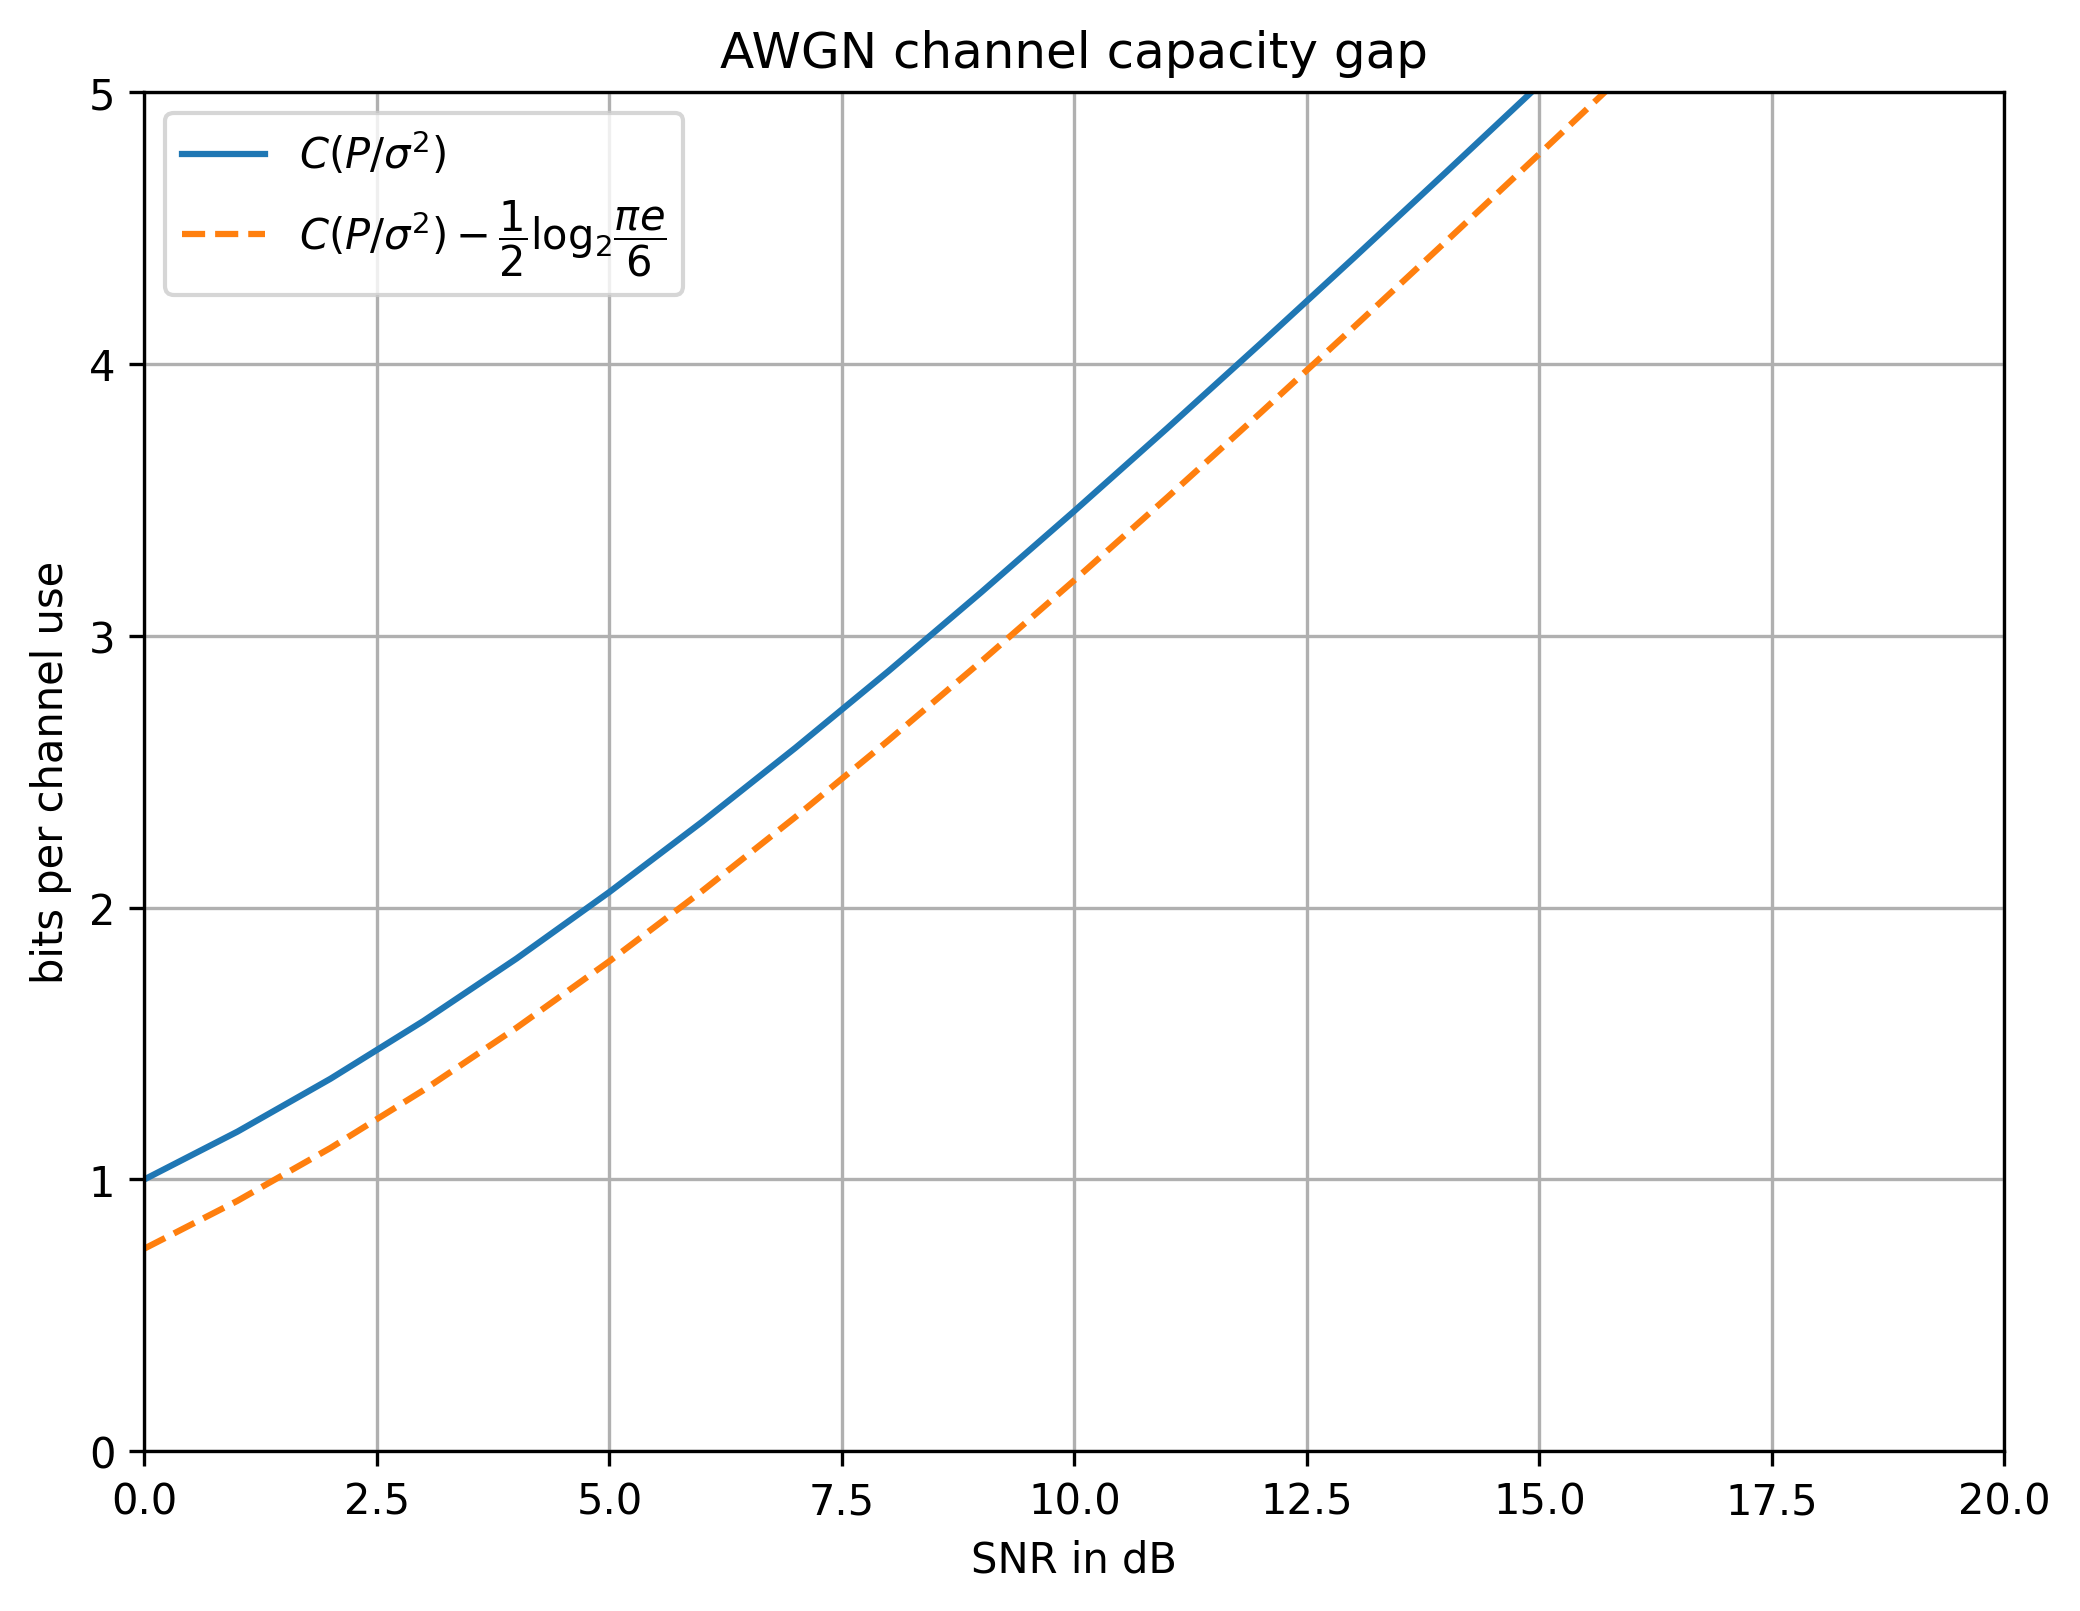
\includegraphics[width=\textwidth]{figs/capacity_gap.png}
	\caption{AWGN channel capacity gap. The orange line indicates the upper capacity bound for any uniformly distributed constellation.}
    \label{fig:capacity_gap}
\end{figure}
To show that the shaping gap is tight, it is necessary to proof an upper bound for $\mathbb{I}(X_u;Y_u)$ that approaches \ref{eqn:gap} with increasing \cgls{snr}. We refer the reader to \cite{BoechererCM}, Section 4.3, for this proof.
\subsection{Uniform Discrete Input Bound}
We now show the penalty received for the use of an equidistant M-\cgls{ask} constellation. We define the constellation points as
\begin{align}
	\mathcal{X} = \{\pm\Delta 1, \pm\Delta 3,\dots, \Delta(M-1)\},
\end{align}
where $\Delta$ is the scaling factor of the constellation, so that the channel input is $X$. If $X_M$ is uniformly distributed, the resulting power  is
\begin{align}
	P = \mathbb{E}\left[X_{M}^2\right] = \Delta^2\frac{M^2 - 1}{3}.
\end{align}
\begin{theorem}[Uniform Discrete Input Bound]
\label{th:uniform_discrete_input_bound}
The mutual information achieved by $X_M$ is lowered bounded by
\begin{align}
\mathbb{I}(X_M;Y_M) &\geq \dfrac{1}{2} \log_2 \left( \dfrac{M^2}{M^2 -1}\right) - \dfrac{1}{2} \log_2 \left[2\pi e\left( \dfrac{P}{M^2 -1}+ \dfrac{P}{1+P/\sigma^2}\right)\right]\\
& < C(\text{snr}) - \dfrac{1}{2} \log_{2} \left(\dfrac{\pi e}{6}\right) - \dfrac{1}{2} \log_2 \left[1 +\left(\dfrac{2^{C(\text{snr})}}{M}\right)^2\right]\\
& < C(\text{snr}) - \text{Penalty}(\text{Uniform dist.}) - \text{Penalty}(\text{Equidistant dist.})
\end{align}
where $\text{snr} = P/\sigma^2$.
\end{theorem}
We refer the reader to \cite{BoechererCM}, section 4.5, for the proof.
Theorem \ref{th:uniform_discrete_input_bound} shows our goal, namely that both the usage of a uniform distribution and an equidistant constellation penalizes the capacity. We can additionally compute the relation between the constellation size, $M$, and $C(\text{snr})$ so that the resulting \cgls{mi} is within a constant gap of capacity. To make this result even more attractive, we increase the constraint for the gap to match the order of the distribution loss (0.255 bits). We obtain
\begin{align}
	- \dfrac{1}{2} \log_2 \left[1 +\left(\dfrac{2^{C(\text{snr})}}{M}\right)^2\right] \leq - \dfrac{\log_2 e}{2} \left(\dfrac{2^{C(\text{snr})}}{M}\right)^2 = \dfrac{1}{4}\\
	\Leftrightarrow M = 2^{C(\text{snr}) + \tfrac{1}{2}+\tfrac{1}{2} \log_2 \log_2 e}
\end{align}
by using $\log_e(x)\leq (1-x)$. So if 
\begin{align}
	\log_2 M \approx C(\text{snr}) +0.77,
\end{align}
then the mutual information is within 0.5 bit of capacity.

% Write about Maxwel-Boltxman distributions...
\subsection{Capacity-achieving distributions}
We now address the question of finding the discrete probability distribution which maximizes the capacity. Such distribution should be free of the $ \dfrac{1}{2} \log_{2} \left(\dfrac{\pi e}{6}\right)$ penalty. We use again an \cgls{ask} constellation with M signal points ( in practice, M is a power of 2) given by 
\begin{align}
	\mathcal{X} = \{\pm 1, \pm 3,\dots, (M-1)\}.
\end{align}

Let $X$ be a random variable with distribution $P_X$ over $\mathcal{X}$. As before, we scale $X$ by a $\Delta > 0$ and the resulting input/output relation for an \cgls{awgn} channel becomes
\begin{align}
	Y = \Delta X + Z
\end{align}

In consequence, the \cgls{mi} of the channel input and output is 
\begin{align}
	\mathbb{I}(\Delta X; Y) &= \mathbb{I}(\Delta X; \Delta X + Z)\\
	&= \mathbb{I}(\Delta X; \Delta X + Z)
\end{align}

where the second equality follows because $(\Delta X)$ is a deterministic function of $X$ and vice-versa. Under an input average power constraint $P$, the scaling $\Delta$ and the distribution $P_X$ must be chosen to satisfy
\begin{align}
	\mathbb{E}[(\Delta X)^2] \leq P.
\end{align}

Formally, our optimization problem is the following

\begin{align}
	C(P/\sigma^2) &= \max\limits_{\Delta, P_X :\mathbb{E}[(\Delta X)^2] \leq P} \mathbb{I}(X;\Delta X+Z).
\end{align}

Maximizing the mutual information $\mathbb{I}(X;\Delta X+Z)$ both over the scaling of the constellation points and the input distribution requires a relatively high amount of power. Instead, as shown in \cite{BoechererCM}, section 5.3, we will use a sub-optimal input distribution which follows from maximizing the input entropy.

We expand the mutual information as
\begin{align}
	\mathbb{I}(X,\Delta X+Z) &= \mathbb{H}(X) - \mathbb{H}(X| \Delta X+Z)
\end{align}
and fixing $\Delta$, we select the input distribution $P_{X_\Delta}$ that maximizes the input entropy under our power constraint, i.e., we choose
\begin{align}
	P_{X_\Delta} &= \argmax\limits_{P_X:\mathbb{E}[(\Delta X)^2] \leq P} \mathbb{H}(X).
\end{align}
Without the discrete constraint, the solution would be a Gaussian distribution. For this reason we explore sampled Gaussian distributions, also known as \cgls{mb} distributions. For each $\mathcal{X} = \{\pm1, \pm 3,\dots, (M-1)\}$, define
\begin{align}
	P_{X_v}(x_i) &= A_{\nu}e^{-\nu{x_i}^2},\text{  } A_{\nu} = \dfrac{1}{\sum\limits_{i=1}^{M}e^{-\nu{x_i}^2}} 
\end{align}

We now show that $P_{X_\Delta}$ is given by
\begin{align}
P_{X_\Delta}(x_i) = P_{X_\nu}(x_i) \text{ with } \nu : \mathbb{E}[(\Delta X_{\nu})^2] = P
\end{align}

\begin{proof}
Consider the finite set $\mathcal{X} = {x_1, x_2, \dots , x_n}$ . Let $f$ be a function that
assigns to each $x_i \in \mathcal{X}$ a positive cost $f(x_i) > 0$. Define the \cgls{mb} distribution
\begin{align}
	P_{X_v}(x_i) &= A_{\nu}e^{-\nu f(x_i)},\text{  } A_{\nu} = \dfrac{1}{\sum\limits_{i=1}^{M}e^{-\nu f(x_i)}} 
\end{align}	
Let $P_X$ be some distribution on $\mathcal{X}$ with $ \mathbb{E}[f(X)] = P $. Choose $\nu : \mathbb{E}[f(X_{\nu})] = P$
\begin{align}
	0 &\leq \mathbb{D}(P_X \Vert P_{X_{\nu}})\\
	&= \sum\limits_{x \in \text{Support}(P_{X_{\nu}})} P_X \log(\dfrac{P_X(x)}{P_{X_{\nu}}(x)}) \\
	&= -\mathbb{H}(X) - \sum\limits_{x \in \text{Support}(P_{X_{\nu}})} P_X(x) \log(P_{X_{\nu}}(x)) \\
	&\overset{\text{(*)}}{=} -\mathbb{H}(X) - \sum\limits_{x \in \text{Support}(P_{X_{\nu}})} P_{X_{\nu}}(x) \log(P_{X_{\nu}}(x)) \\
	&= -\mathbb{H}(X) + \mathbb{H}(X_{\nu}) \\
	\mathbb{H}(X) &\leq \mathbb{H}(X_{\nu})
\end{align}
where the (*) marked step follows since both distributions produce the same moments for $log(P_{X_{\nu}}(x))$.
\end{proof}


	
\section{Autoencoders}
In the following we consider \cglspl{ffnn}, an specific type of \cgls{nn}, \cgls{sgd}, and autoencoders.

\subsection{Feed-Forward Neural Networks}
\cGlspl{ffnn} are structures which map an input vector $\bold{v_0} = (v_{0,1} \dots v_{0,M})$ to an output vector $\bold{v_k} = (v_{K,1} \dots v_{K,N})$, i.e., $\bold{v_K}=f_{\text{NN}}(\bold{v_0})$. This transformation is accomplished by composing functions, which in turn are computed by layers. The number of layers, K, is commonly referred to as depth of the network. And each layer can be composed of a specific number of units (neurons), M, often referred to as width of the layer. A representation of this structure is shown in Figure \ref{fig:ffnn}

\begin{figure}[H]
	\centering
	\tikzset{
    neuron/.style={
		circle,
		draw=black,
		minimum size=0.8cm,
		fill=gray,
	},	
    neuron dark/.style={
		circle,
		draw=black,
		minimum size=0.8cm,
		fill=TUMBlueDark,
	},	
	neuron missing/.style={
		draw=none, 
		fill=white,
		scale=1.0,
		text height=0.3cm,
		execute at begin node=\color{black}$\vdots$
	},
	neuron sigma/.style={
		circle,
		draw=black,
		fill=white,
		scale=1.0,
%		text height=0.5cm,
		execute at begin node=\color{black}$\Sigma$
	},	
	label/.style = {draw=none, fill=none, rectangle, minimum height=1em, minimum width=1em},
	blockrx/.style = {draw, fill=white, rectangle, minimum height=1.5em, minimum width=6.25em},
	blocktx/.style = {draw, fill=white, rectangle, minimum height=1.5em, minimum width=13em},
	block/.style = {draw, fill=white, rectangle, minimum height=2em, minimum width=10em,rounded corners},
	blockthesis/.style = {draw, fill=gray!20, rectangle, minimum height=1.5em, minimum width=40em,rounded corners},
	block1/.style = {draw, fill=white, rectangle, minimum height=1.5em, minimum width=1.5em,rounded corners},
	tmp/.style  = {coordinate}, 
	sum/.style= {draw, fill=white, circle, node distance=1cm},
	mul/.style= {draw=none, fill=white, circle, node distance=1cm},
	input/.style = {coordinate},
	output/.style= {coordinate},
	pinstyle/.style = {pin edge={to-,thin,black}
	}
}
\begin{tikzpicture}
	\draw [<->] (-1,1.5) -- (-1,-4) node [left, midway] {$\text{width}_k\equiv M_k$};	

	\draw [dashed] (0,1.5) -- (0,-4) node [yshift=6cm] {input layer};
	
	\foreach \m [count=\y] in {1,missing,3,missing,5}
	\node [neuron/.try, neuron \m/.try] (input1-\y) at (0,2-\y*1.1) {};
	
	\draw [dashed] (2,1.5) -- (2,-4) node [yshift=6cm] {k-layer};
	
	\foreach \m [count=\y] in {1,2,missing,4}
	\node [neuron/.try, neuron \m/.try ] (hidden1-\y) at (2,1.8-\y*1.1) {};
	
	\draw [dashed] (4,1.5) -- (4,-4) node [yshift=6cm] {input layer};	
	
	\foreach \m [count=\y] in {1,2}
	\node [neuron/.try, neuron \m/.try ] (output1-\y) at (4,0.4-\y*1.1) {};
	
	\draw [<->] (0,-4.2) -- (4,-4.2) node [below, midway] {depth$\equiv K$};	

	%mesh1
	\foreach \i in {1,3,5} 
	\foreach \j in {1,2,4}
	\draw [->] (input1-\i) -- (hidden1-\j);
	
	
	\foreach \i in {1,2,4}
	\foreach \j in {1,2}
	\draw [->] (hidden1-\i) -- (output1-\j);
	
\end{tikzpicture}
	\caption{Representation of the structure of a \cgls{ffnn}.}
	\label{fig:ffnn}
\end{figure}


Note that the width of the input and output layers must match the dimensions of the input and output vectors.\\
Mathematically, the output of a unit is parameterized by a weight, $\bold{w}_{k,m}$, and a bias, $b_{k,m}$, and can be expressed as
\begin{align}
	v_{k,m} = g_{\text{NL},k}(\vb{v}_{k-1}\vb{w}^\top_{k,m} + b_{k,m}), \qquad k = 1, \dots, K \qquad m = 1, \dots, M.
	\label{eqn:neuron}
\end{align}
Where in (\ref{eqn:neuron}), k indicates the layer index, m indicates the unit index, and $g_{\text{NL},k}(\cdot)$ is a nonlinear function, e.g., \cgls{relu}, applied between layers.

\begin{figure}[H]
\tikzstyle{unit}=[draw,shape=circle,minimum size=1.15cm]
\centering
\begin{tikzpicture}[shorten >=1pt,->]
	\node[unit](p) at (2,1){$\Sigma$};
	\node(dots) at (-0.25,1){\vdots};

	\draw (2,2) node[yshift=10]{$b_{k,n}$} -- (p);
	
	\draw (-0.75,1.75) node[xshift=-20]{$v_{k-1,1}$} --(p);
	\draw (-0.75,1.75) node[xshift=1.2cm]{$w_{k-1,1}$} --(p);
	
	\draw (-0.75,0) node[xshift=-20]{$v_{k-1,M}$} -- (p);
	\draw (-0.75,0) node[xshift=1.2cm]{$w_{k-1,M}$} -- (p);
	
	\node[unit, scale=0.6](f) at (3.5,1){$g_{\text{NL},k}$};
	
	\draw (p) -- (f);
	\draw (f) -- (4.5,1) node[xshift=10]{$v_{k,m}$};
\end{tikzpicture}
\caption{Diagram for the output's computation of a single unit as (\ref{eqn:neuron}).}
\end{figure}
Indeed, without the nonlinear function the \cgls{ffnn} lacks the expressive power required to approximate any function \cite{HORNIK1989359}.\\
Finally, using matrix notation we can express the output of each layer as
\begin{align}
	\vb{v_k} = g_{\text{NL},k}(\vb{W}_k\vb{v}_{k-1}+\vb{b}_k), \qquad k = 1, \dots, K.
\end{align}

These structures, together with a training algorithm, help us to find parameters $\bold{W_k}$ and $\bold{b_k}$ such that $f_{\text{NN}}(\bold{v_0})$ approximates an unknown function. To this end, the algorithm receives training sets of observed pairs of the unknown function, where each pair has the form $\{$input, output$\}$.

\subsection{Stochastic Gradient Descent}
To find fitting sets of parameters $\{\bold{W_k}, \bold{b_k}\}$ we define a loss function,  $L(\bold{W_k} , \bold{b_k})$, that compares the current output of the \cgls{nn} with the desired output from the training set. The most used algorithm is \acrfull{sgd} which starts with a random set of initial values and then updates any trainable parameter, $\theta$, with each iteration as
\begin{align}
	{\theta}_{new} = {\theta}_{old} + \epsilon \grad L({\theta}_{old}) %, \qquad \boldsymbol{\theta} \in \{\bold{W_k}, \bold{b_k}\}
\end{align}
where, $\grad$ is the gradient, and $\epsilon$ stands for the learning rate. To compute the gradient efficiently a computational graph stores the transformations to the factors which influenced the loss function. 

\subsection{Autoencoders}
Autoencoders have been very successful in fields like information compression, dimensionality reduction or computer vision. In the context of \cgls{ml} and communication systems it was pioneered by \citet{O'Shea}. The idea behind an autoencoder is to transmit a particular representation of the input data so that at the output, it can be reconstructed with minimal error. This means that the desired representations must be robust with respect to the channel impairments (i.e. noise, fading, distortion, etc.), referred to as the \textit{bottleneck} in the autoencoder jargon. To find such representations and the corresponding mappings, $\textbf{x}$ to $\textbf{y}$, we make use of two \cglspl{ffnn}: the encoder, performing $f(\textbf{x})$, and the decoder, performing $g(\textbf{y})$. %Figure \ref{fig:autoencoder} ilustrates these concepts.

\begin{figure}[h]
\centering
\tikzset{
    neuron/.style={
		circle,
		draw=black,
		minimum size=0.4cm,
		fill=gray,
	},	
    neuron dark/.style={
		circle,
		draw=black,
		minimum size=0.4cm,
		fill=TUMBlueDark,
	},	
	neuron missing/.style={
		draw=none, 
		fill=white,
		scale=1.0,
		text height=0.3cm,
		execute at begin node=\color{black}$\vdots$
	},
	label/.style = {draw=none, fill=none, rectangle, minimum height=1em, minimum width=1em},
	blockrx/.style = {draw, fill=white, rectangle, minimum height=1.5em, minimum width=6.25em},
	blocktx/.style = {draw, fill=white, rectangle, minimum height=1.5em, minimum width=13em},
	block/.style = {draw, fill=white, rectangle, minimum height=2em, minimum width=10em,rounded corners},
	blockthesis/.style = {draw, fill=gray!20, rectangle, minimum height=1.5em, minimum width=40em,rounded corners},
	block1/.style = {draw, fill=white, rectangle, minimum height=1.5em, minimum width=1.5em,rounded corners},
	tmp/.style  = {coordinate}, 
	sum/.style= {draw, fill=white, circle, node distance=1cm},
	mul/.style= {draw=none, fill=white, circle, node distance=1cm},
	input/.style = {coordinate},
	output/.style= {coordinate},
	pinstyle/.style = {pin edge={to-,thin,black}
	}
}
\begin{tikzpicture}
	%encoder
	\node[text width=3cm] at (1.5,2) {Encoder $f(\textbf{x})$};
	
	
	\draw [dashed] (2.6,1.3) -- (2.6,-1.5);
	
	\foreach \m [count=\y] in {1,missing,3,missing,5}
	\node [neuron/.try, neuron \m/.try] (input1-\m) at (0,2-\y*0.7) {};
	
	\foreach \m [count=\y] in {1,2,missing,4}
	\node [neuron/.try, neuron \m/.try ] (hidden1-\m) at (1,1.8-\y*0.7) {};
	
	\foreach \m [count=\y] in {1,2,missing,4}
	\node [neuron/.try, neuron \m/.try ] (hidden2-\m) at (1.8,1.8-\y*0.7) {};
	
	\foreach \m [count=\y] in {1,2}
	\node [neuron/.try, neuron \m/.try ] (output1-\m) at (2.6,1-\y*0.7) {};
	
	\node[text width=0.2cm] at (-1,-0.1) {$\textbf{x}$};
	
	
	\foreach \i in {1,3}
	\draw [<-] (input1-\i) -- ++(-0.6,0);
	
	\draw [->] (output1-1) -- ++(1.8,0);
	\draw [->] (output1-2) -- ++(1.8,0)
	node [below, midway] {\textit{bottleneck}};
	
	
	\draw [<-] (input1-5) -- ++(-0.6,0);

	%mesh1
	\foreach \i in {1,3,5} 
	\foreach \j in {1,2,4}
	\draw [->] (input1-\i) -- (hidden1-\j);
	
	\foreach \i in {1,2,4}
	\foreach \j in {2}
	\draw [->] (hidden1-\i) -- (hidden2-\j);
	
	\draw [->] (hidden1-2) -- (hidden2-1); 
	\draw [->] (hidden1-4) -- (hidden2-1); 
	
	\draw [->] (hidden1-1) -- (hidden2-4); 
	\draw [->] (hidden1-2) -- (hidden2-4); 
	
	\foreach \i in {1,2,4}
	\foreach \j in {1,2}
	\draw [->] (hidden2-\i) -- (output1-\j);
	
	\draw [dashed] (4.6,1.3) -- (4.6,-1.5);
	
	%decoder
	\node[text width=3cm] at (6.8,2) {Decoder $g(\textbf{y})$};
	\foreach \m [count=\y] in {1,2}
	\node [neuron/.try, neuron \m/.try ] (input2-\m) at (4.6,1-\y*0.7) {};
	
	\foreach \m [count=\y] in {1,2,missing,4}
	\node [neuron/.try, neuron \m/.try ] (hidden3-\m) at (5.4,1.8-\y*0.7) {};
	
	\foreach \m [count=\y] in {1,2,missing,4}
	\node [neuron/.try, neuron \m/.try ] (hidden4-\m) at (6.2,1.8-\y*0.7) {};
	
	\foreach \m [count=\y] in {1,missing,3,missing,5}
	\node [neuron/.try, neuron \m/.try] (output2-\m) at (7,2-\y*0.7) {};
	
	%outputs
	\foreach \i in {1,3,5}
	\draw [->] (output2-\i) -- ++(0.6,0);
	
	%mesh2
	\foreach \i in {1,2} 
	\foreach \j in {1,2,4}
	\draw [->] (input2-\i) -- (hidden3-\j);
	
	\foreach \i in {1,2,4}
	\foreach \j in {2}
	\draw [->] (hidden3-\i) -- (hidden4-\j);
	
	\draw [->] (hidden3-2) -- (hidden4-1); 
	\draw [->] (hidden3-4) -- (hidden4-1); 
	
	\draw [->] (hidden3-1) -- (hidden4-4); 
	\draw [->] (hidden3-2) -- (hidden4-4); 
	
	\foreach \i in {1,2,4}
	\foreach \j in {1,3,5}
	\draw [->] (hidden4-\i) -- (output2-\j);
	
	\node[text width=0.2cm] at (8,-0.1) {$\hat{\textbf{x}}$};
	
	
	
	
\end{tikzpicture}
\caption{Representation of the \cglspl{nn} of an autoencoder.}
\label{fig:autoencoder}
\end{figure}

One particular requirement for using \cgls{sgd} in autoencoders is that the loss gradient needs to be backpropagated all the way through receiver and channel to the transmitter. Otherwise, the transmitter parameters cannot be updated. This in turn means, that the end-to-end path must be available as differentiable functions during training.
\section{Outlook}
We can now set up the problem which we would like to address in this work. Namely, to train a \cgls{nn}-based autoencoder system which can find the optimal distribution and location of the  to-be-transmitted constellation. By maximizing the \cgls{mi} during training, the output distribution must satisfy (\ref{eq:C_minus_D}), and thus, approach the channel capacity without the mentioned penalties. Because \cglspl{nn} are universal function approximators \cite{HORNIK1989359}, this technique is paramount for finding the appropriate parameters over channels with a very complex, or even mathematically intractable, model.
%!TEX root = ../main.tex
\chapter{Contribution}\label{chap:contribution}
\section{Notation}
In the following we will use the notation:
\begin{align*}
	\mathbb{I} \left(X , Y; D, P_M, C_M \right)
\end{align*}
which expresses the mutual information between $X$ and $Y$ and $D, P_M, C_M$, separated by a semi-colon, are the trainable parameters of the system. The parameters can be seen as additional input to a function.
\section{First implementation}
In this section we break-down the autoencoder system presented by \citep{Aref} et. al. in \cite{Aref}.
\subsection{Optimization of trainable parameters}
As we have seen in chapter \ref{chap:preliminaries}, the goal of probabilistic constellation shaping is to maximize the mutual information
\begin{align}
	 \max_{D, P_M, C_M} \mathbb{I} \left(X , Y ; D, P_M, C_M \right) \overset{\text{(a)}}{=} \mathbb{H}(X) - \mathbb{X}(P_{X|Y} \Vert Q_{X|Y} ; D, P_M, C_M)
\end{align}

where the entropy is maximized when the symbols probabilities follow a \cGls{mb} distribution; and the cross-equivocation is minimum when $Q_{X|Y} = P_{X|Y}$.

Typically, the gradient descent (or ascent, as we intent to maximize) allows us to solve the optimization problem by adjusting the trainable parameters as:
\begin{align}
	\theta_{new} = \theta_{old} + \epsilon \pdv{\theta_{old}} \mathbb{I} \left(X , Y ; \theta_{old} \right)
\end{align}
for all trainable parameters $\theta \in P_M, C_M, D$. And the \cGls{mi} can be numerically approximated by
\begin{align}
	\mathbb{I} \left(X , Y\right) \approx \mathbb{I} \left(X , Y\right)_{\text{num}} &= \dfrac{1}{B} \sum \limits_{i = 1}^{B} - \log_2(P(x_i)) + \log_2(Q_{X|Y}(x_i|y_i))\\
	&= \dfrac{1}{B} \sum \limits_{i = 1}^{B} L(x_i, y_i).
\end{align}

Next, the following approximation usually allows to adjust the trainable parameters:
\begin{align}
	\pdv{\theta} \mathbb{I} \left(X , Y ; \theta \right) \approx \pdv{\theta} \mathbb{I} \left(X , Y\right)_{\text{num}} = \dfrac{1}{B} \sum \limits_{i = 1}^{B} L(x_i, y_i).
\end{align}

However, \citep{Aref} claims that although this is true for the constellation locations $(\theta \in C_M)$ and the demapper parameters $(\theta \in D)$, it does not hold for the constellation probabilities $\{p_1, p_2, \dots, p_M\} = P_M$
\begin{align}
\label{eqn:mi_pdv_p}
	\pdv{p_j} \mathbb{I} \left(X , Y ; P_M \right) \not\approx \dfrac{1}{B} \sum \limits_{i = 1}^{B} \pdv{p_j} L(x_i, y_i)
\end{align}

as $\{p_1, p_2, \dots, p_M\}$ changes the statistics of the training set.

For this reason, \ref{eqn:mi_pdv_p} must be computed differently. On the one hand, to compute the derivative of the cross-equivocation, the following expansions are useful
\begin{align}
	\mathbb{X}\left(P_{X|Y} \Vert Q_{X|Y} \vert Y=b \right) = \sum \limits_{a \in Supp(P_{X|Y}(\cdot|b))} P_{X|Y}(a|b) \log_2(Q_{X|Y}(a|b))
\end{align}

\begin{align}
	\mathbb{X}\left(P_{X|Y} \Vert Q_{X|Y}\right) = \sum \limits_{b \in Supp(P_Y)} P_Y(b) \mathbb{X}\left( P_{X|Y} \Vert Q_{X|Y} \vert Y=b \right) 
\end{align}

as combined together and applying Bayes' theorem they yield

\begin{align}
\label{eqn:CE_expanded}
	\mathbb{X}\left(P_{X|Y} \Vert Q_{X|Y}\right) = \sum \limits_{(a,b) \in Supp(P_{XY})} P_X(a) P_{Y|X}(b|a) \log_2(Q_{X|Y}(a|b)). 
\end{align}

And so, the derivative results
\begin{align}
	\pdv{p_j} \mathbb{X}\left(P_{X|Y} \Vert Q_{X|Y}\right) &= \sum \limits_{b \text{ if } x=j} P_{Y|X}(b|j) \log_2 Q_{X|Y}(j|b) \\
	& + \sum \limits_{(a,b) \in Supp(P_{XY})} P_{XY}(a, b) \pdv{p_j} \log_2 Q_{X|Y}(a|b)
\end{align}
which can be rewritten using the expectation operator as
\begin{align}
	\pdv{p_j} \mathbb{X}\left(P_{X|Y} \Vert Q_{X|Y}\right) &= \mathbb{E}_{Y|X}[ \log_2 Q_{X|Y}(j|b)| X=j] \\
	& + \mathbb{E}_{XY}[ \pdv{p_j} \log_2 Q_{X|Y}(a|b)].
\end{align}
The terms can now be numerically computed as
\begin{align}
\label{eqn:CE_term_1}
	\mathbb{E}_{Y|X}[ \log_2 Q_{X|Y}(j|b)| X=j] \approx \dfrac{1}{Bp_j}\sum \limits_{b \text{ if } x=j} \log_2 Q_{X|Y}(j|b)
\end{align}
\begin{align}
\label{eqn:CE_term_2}
	\mathbb{E}_{XY}[ \pdv{p_j} \log_2 Q_{X|Y}(a|b)] \approx \dfrac{1}{B} \sum \limits_{(a,b) \in Supp(P_{XY})} \log_2 Q_{X|Y}(a|b).
\end{align}
On the other hand, the derivative of the entropy w.r.t. $p_j$ is
\begin{align}
\label{eqn:H_term_1}
	\pdv{p_j} \mathbb{H}(X) = \pdv{p_j} \sum \limits_{i = 1}^{B} - p_i \log_2(p_i) = - \log_2 (p_j) - log_2 (e).
\end{align}

Now, combining \ref{eqn:CE_term_1}, \ref{eqn:CE_term_2}, and \ref{eqn:H_term_1} the derivative of the mutual information w.r.t. $p_j$, \ref{eqn:mi_pdv_p}, can be computed as
\begin{align}
	\pdv{p_j} \mathbb{I} \left(X , Y ; P_M \right) \approx - \log_2 (p_j) - \log_2 (e) + \dfrac{1}{Bp_j}\sum \limits_{b \text{ if } x=j} \log_2 Q_{X|Y}(j|b) + \dfrac{1}{B} \sum \limits_{(a,b)} \log_2 Q_{X|Y}(a|b)
\end{align}

\citep{Aref} now indicates that the following terms can be computed via backpropagation
\begin{align}
	- \log_2 (p_j) + \dfrac{1}{Bp_j}\sum \limits_{b \text{ if } x=j} \log_2 Q_{X|Y}(j|b) = \dfrac{1}{B} \sum \limits_{i = 1}^{B} \pdv{p_j} L(x_i, y_i)
\end{align}
while the remaining ones must be explicitely computed and added to the gradient after backpropagating. We call this step \textit{gradient correction} and it is due to the change of statistics in the sampled batch.

%\input{chapters/simulation}
%\input{chapters/conclusions}

\cleardoubleemptypage



% ########
% Appendix
% ########
\appendix
%!TEX root = ../main.tex
\addchap{Appendix A}\label{chap:appA} % basically chapter*, but keeps the chapter in the table of contents
First appendix goes here.

%!TEX root = ../main.tex
\addchap{Appendix B}\label{chap:appB} % basically chapter*, but keeps the chapter in the table of contents
Second appendix goes here.


% ### list of acronyms (comment out if does not work and you don't want to make it work)
\printglossary[
    type = acronym,
    title = List of Abbreviations,
    toctitle = List of Abbreviations,
    style = long,
    nonumberlist,
    numberedsection = false,
]

% ### bibliography
% Use IEEE DIN 1505 style for bibliography
\bibliographystyle{IEEEtranSA}
%\nocite{*} % include all references without checking (don't do this)
\bibliography{refs}
\end{document}

%
% EOF!
%
%%% Local Variables:
%%% mode: latex
%%% TeX-master: t
%%% End:
